\documentclass[14pt,a4paper]{article}
\usepackage[14pt]{extsizes}
\usepackage[left=1.5cm, right=1.5cm, top=1.5cm, bottom=1.5cm]{geometry}
\usepackage[utf8]{inputenc}
\usepackage[T2A]{fontenc}
\usepackage[english, russian]{babel}
\usepackage{amsmath,amsfonts,amssymb,amsthm,mathtools} 
\usepackage{amsfonts}
\usepackage{amssymb}
\usepackage{titleps}
\usepackage{hyperref}
\usepackage{float}
\usepackage{graphicx}
\usepackage{multirow}
\usepackage{hhline}
\usepackage{wrapfig}
\usepackage{tikz}
\usepackage{pgfplots}
\usepackage{xcolor}
\usepackage{subfig}
\usepackage{upgreek}
\usepackage{bm}
\usepackage{longtable}


\newcommand{\w}[1]{\text{#1}}
\newcommand{\und}[1]{\underline{#1}}
\newcommand{\img}[3]{
	\begin{figure}[H]
	\begin{center}
	\includegraphics[scale=#2]{#1}
	\end{center}
	\begin{center}
 	\textit{#3}
	\end{center}
	\end{figure}
}
\newcommand{\aw}[1]{
	\begin{center}
	\textit{#1}
	\end{center}
	\n
}
\newcommand{\be}[1]{
	\begin{center}
	\boxed{#1}
	\end{center}
}
\newcommand{\beb}[1]{
	\begin{equation}
	\boxed{#1}
	\end{equation}
}
\newcommand{\eb}[1]{
	\begin{equation}
	#1
	\end{equation}
}
\newcommand{\n}{\hfill \break}
\newcommand{\x}{\cdot}
\newcommand{\specialcell}[2][c]{%
	\begin{tabular}[#1]{@{}c@{}}#2\end{tabular}}

\newcommand{\mA}{\; мА}
\newcommand{\uA}{\; мкА}
\newcommand{\uV}{\; мкВ}
\newcommand{\V}{\; В}
\newcommand{\kV}{\; кВ}
\newcommand{\m}{\; м}
\newcommand{\del}{\; дел}
\newcommand{\mm}{\; мм}
\newcommand{\um}{\; мкм}
\newcommand{\nm}{\; нм}
\newcommand{\cm}{\; см}
\newcommand{\dptr}{\; дптр}
	
\begin{document}
\section*{Работа 4.7.2}	
\section*{Эффект Поккельса}
\subsection*{Киркича Андрей, Б01-202, МФТИ}		
\section*{Аннотация}
В работе мы, измерив радиусы интерференционных колец, определили разность показателей преломления $n_o - n_e$; подав на кристалл постоянное напряжение, получили свет, поляризованный по кругу; определили полуволновое напряжение по фигурам Лиссажу на экране осциллографа.
\section*{Экспериментальная установка}

Схема экспериментальной установки приведена на рисунке:

\begin{figure}[H]
	\centering
	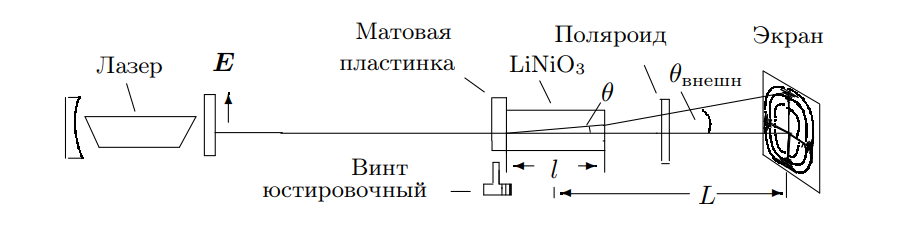
\includegraphics[width=0.8\textwidth]{Изображения/ust.png}
	\caption{Схема эксперимента}
\end{figure}

\begin{figure}[H]
	\centering
	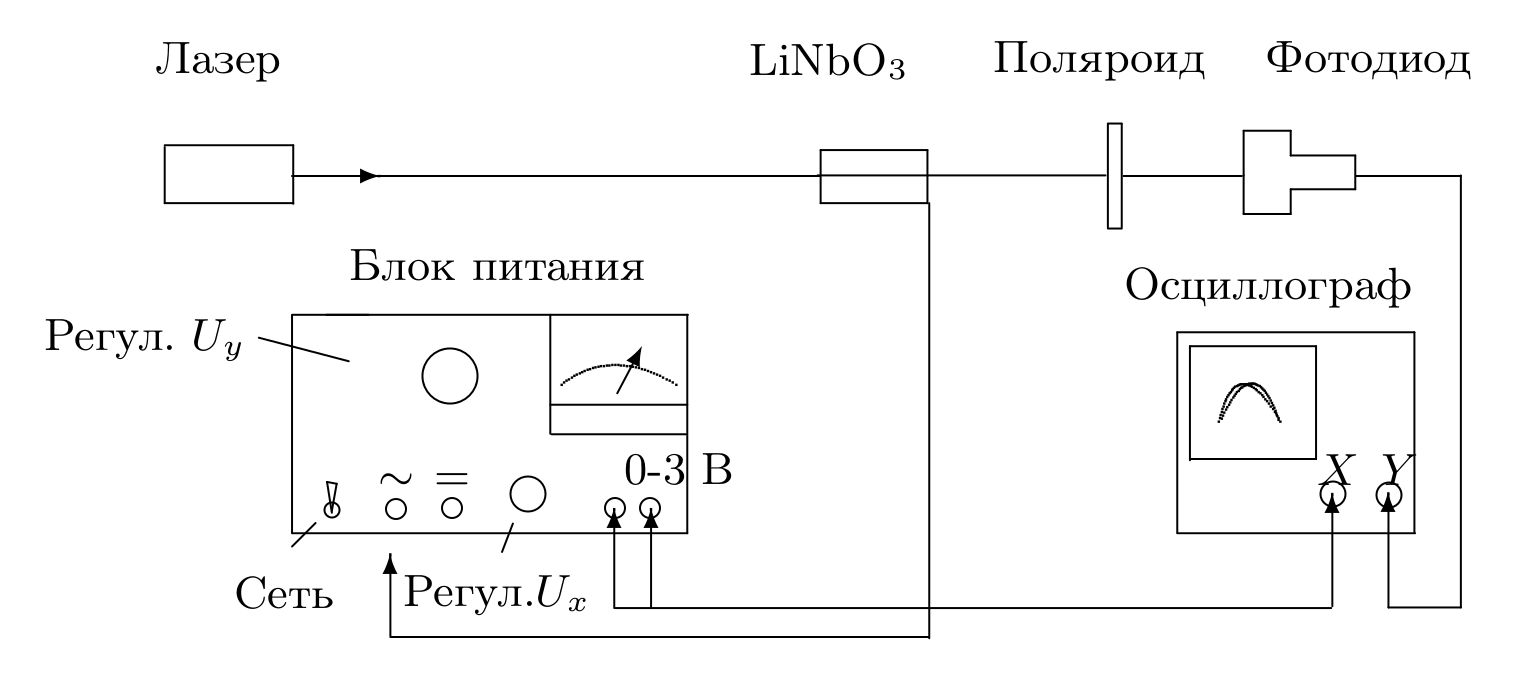
\includegraphics[width=0.8\textwidth]{Изображения/facility.png}
	\caption{Схема экспериментальной установки}
\end{figure}
\n
Параметры установки:
\begin{itemize}
\item Длина волны $\lambda = 630$ нм
\item Показатель преломления для обыкновенной волны $n_o = 2.29$
\item Длина кристалла $l = 25$ мм
\item Поперечный размер кристалла $d = 3$ мм
\item Цена деления шкалы прибора $1$ дел $= 15$ В.
\end{itemize}
\n
Луч света от лазера со встроенным вертикальным поляризатором попадает на кювету с кристаллом необата лития. Перед кюветой можно разместить матовую рассеивающую пластинку. Главная оптическая ось кристалла ориентирована вдоль направления распространения луча. После кюветы расположен поляроид. Результат интерференции наблюдается на экране. На кристалл можно подавать высоковольтное постоянное и переменное напряжение с помощью источника напряжения. Если подавать на кристалл переменное напряжение, то для исследования результата интерференции используется фотодиод, выход которого подключается к одному каналу осциллографа. Ко второму входу осциллографа подключается сигнал с источника напряжение.
	
\section*{Результаты измерений}

Сначала мы установили кристалл на расстоянии $L = 80.0 \pm 0.5$ см до экрана, осветили кристалл лазером через матовую пластину и получили на экране интерференционную картину. Лазерный свет поляризован в вертикальной плоскости. Радиусы тёмных колец $r_m$ представлены в таблице ниже. 

\begin{table}[H]
	\centering
\begin{tabular}{|r|r|r|r|r|r|r|}
	\hline
	$m$ & 1 & 2 & 3 & 4 & 5 & 6 \\
	\hline
	$r_m$, мм & 27.5 & 39.5 & 49.5 & 56.5 & 63.5 & 70.5 \\
	\hline
\end{tabular}
\end{table}
\n
По этим данным мы построили график зависимости квадрата радиуса тёмного кольца от его порядкового номера $r^2(m)$.

\begin{figure}[H]
	\centering
	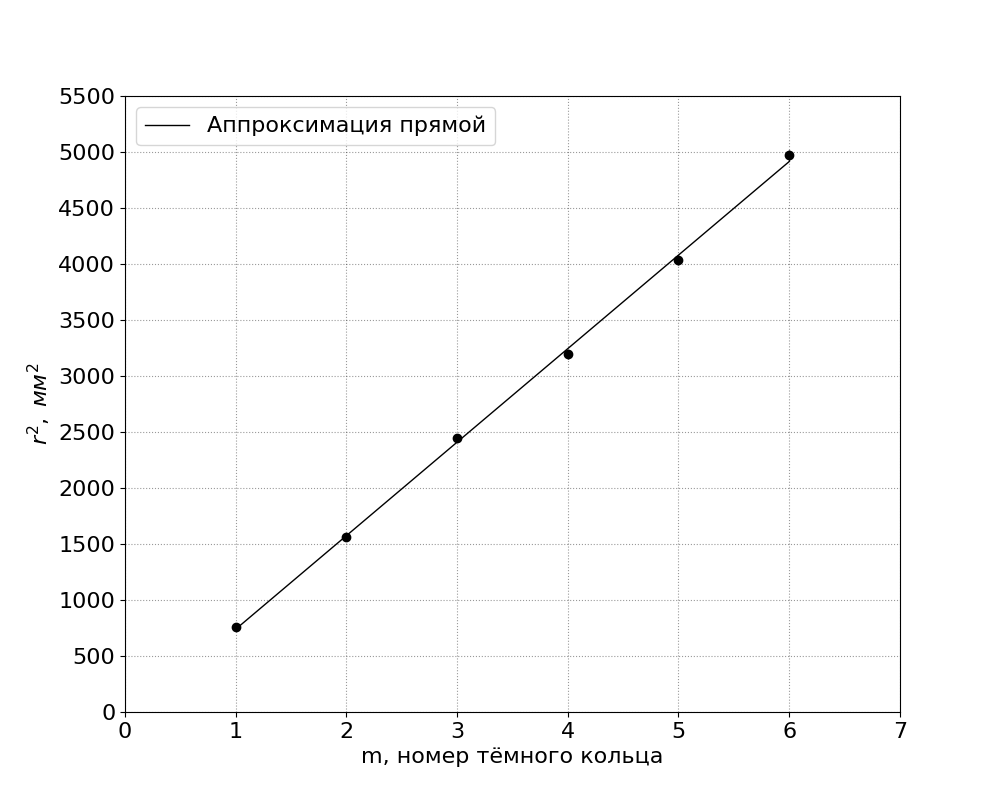
\includegraphics[width=0.5\textwidth]{Графики/r2(m).png}
	\caption{График зависимости $r^2(m)$}
\end{figure}
\n
Данные хорошо сходятся с формулой:
\[r_m = \frac{\lambda}{l} \frac{(n_o L)^2}{n_o - n_e} m\]
\n
Зависимость можно аппроксимировать прямой $y = a x + b$, по углу наклона определить двулучепреломление $n_o - n_e$: \\
\[a = 835 \pm 12 \text{ мм}^2\]
\[b = -95 \pm 47 \text{ мм}^2\]

$$n_o - n_e = \frac{\lambda}{l}\frac{(n_o L)^2}{a} = 0.097 \pm 0.002$$

\subsection*{Определение полуволнового напряжения}
Убедившись, что направление лазерного луча совпадает с направлением на центр интерфереционной картины, мы убрали матовую пластинку. Подключили разъём блока питания на постоянно напряжение, установили регулятор напряжения на минимум и включили блок питания в сеть.
\n\n
Сначала мы определили интересующие нас напряжения без осциллографа. Для этого убрали матовую пластинку. При нулевом напряжении наблюдается минимум интенсивности излучения на экране. Постепенно увеличивая его, мы получали напряжения, соответствующие максимумам и минимумам интенсивности.
\n\n
При перпендикулярных поляризациях лазера и анализатора:
\[U_{\lambda/2} = (270 \pm 15) \text{ В}, \qquad U_\lambda = (630 \pm 15) \text{ В}, \qquad U_{3\lambda/2} = (1020 \pm 15) \text{ В}\]
При паралелльных поляризациях:
\[U_{\lambda/2} = (240 \pm 15) \text{ В}, \qquad U_\lambda = (630 \pm 15) \text{ В}, \qquad U_{3\lambda/2} = (1110 \pm 15) \text{ В}\]
\n
Подав на кристалл напряжение $U_{\lambda/4} = \frac{1}{2}U_{\lambda/2}$ и вращая анализатор, мы убедились, что поляризация круговая.
\n\n
Дальнейшие измерения проводились при помощи осциллографа. Было определено полуволновое напряжение по разности напряжений при максимуме и минимуме у фигуры Лиссажу: $U_{\lambda/2} = \Delta U = 390 \pm 15 \text{ В}$. 
	
\section*{Обсуждение результатов и выводы}
В работе мы наблюдали интерференционную картину обыкновенной и необыкновенной волн, образовавшихся после прохождения кристалла ниобата лития монохроматического поляризованного лазерного излучения.
\n\n
Было измерено двулучепреломление кристалла в отсутствии внешнего электрического поля: 
\[n_o - n_e = 0.097 \pm 0.002.\]
\n
Согласно справочнику для длины волны $\lambda = 632.8$ нм кристалл ниобата лития имеет показатели преломления $n_o = 2.286$, $n_e = 2.203$. Тогда имеем:
\[(n_o - n_e)^{табл} = 0.083.\]
\n
Результаты не сходятся в пределах погрешности, но довольно близки. Расхождение можно объяснить несовершенством лазера - мощность была слабой и из-за этого оценка напряженией на максимумах и минимумах могла быть неточной.
\n\n
В работе было определено полуволновое напряжение образца кристалла ниобата лития $U_{\frac{\lambda}{2}} = (270 \pm 15)$ В методом наблюдения периодических изменений интенсивности света на экране при постоянном внешнем электрическом поле внутри пластинки. 
\n\n
Методом наблюдения фигур Лиссажу при переменном электрическом поле внутри пластинки мы получили значение $U_{\frac{\lambda}{2}} = (390 \pm 15)$ В.
\n\n
Результаты, полученные двумя разными методами, не совпадают. Это можно объяснить большой чуствительностью осциллографа к внешним воздействиям.
\end{document}